\subsection{Adjustable Positive Voltage Regulator:}

\begin{tasks}
\task LM317 circuit with variable resistor in his lower value:
\begin{figure}[H]
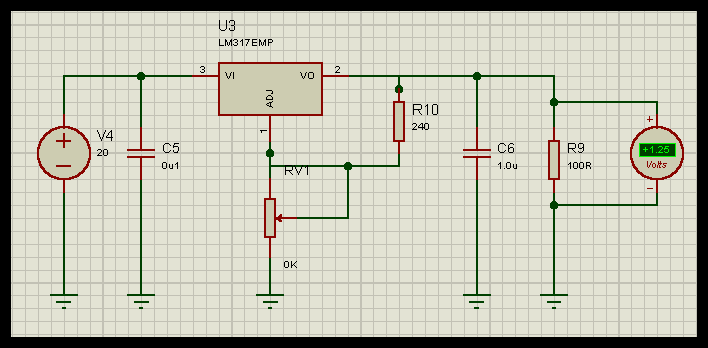
\includegraphics[scale=.6]{min1.png}
\centering \linebreak \linebreak Figure 4.4.0: 0K resistor in adjustable positive voltage regulator circuit.
\end{figure}

\begin{ceqn}
\begin{align}
V_{0_{min}} = 1.25 V
\end{align}
\end{ceqn}

\task LM317 circuit with variable resistor in his maximum value:
\begin{figure}[H]
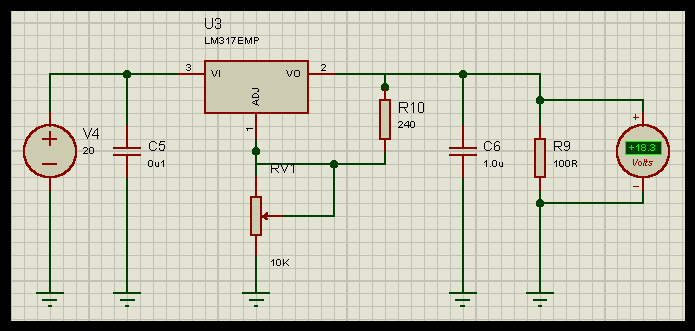
\includegraphics[scale=.6]{max1.png}
\centering \linebreak \linebreak Figure 4.4.1: 10K resistor in adjustable positive voltage regulator circuit.
\end{figure}

\begin{ceqn}
\begin{align}
V_{0_{max}} = 18.3 V
\end{align}
\end{ceqn}
\end{tasks}

\pagebreak